\chapter{Critical Systems}


\begin{figure}[ht]
    \centering
    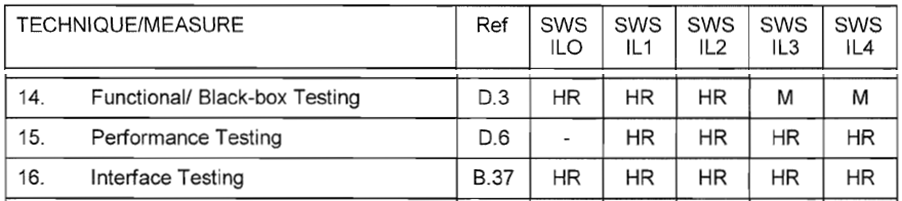
\includegraphics[width=0.9\textwidth]{figures/en-50128-example-recommended-techniques}
    \caption{Example: Recommendation of techniques in EN 50128}
    \label{fig:overview:en-50128-technique-recommendation}
\end{figure}

\section{Hungarian terms}

\begin{table}
    \centering
    \small
    \caption{Hungarian terms for critical systems}
    \begin{tabular}{ll}
        \toprule
        \textbf{English} & \textbf{Hungarian} \\
        \midrule
        assessor & értékelő \\
        availability & rendelkezésre állás \\
        certification & tanúsítvány \\
        fault tolerance & hibatűrés \\
        reliability & megbízhatóság \\
        risk & kockázat \\
        safety & biztonságosság \\
        safety integrity level & biztonságintegritási szint \\
        safety-critical system & biztonságkritikus rendszer \\
        standard & szabvány \\
        tolerable hazard rate & elviselhető veszélygyakoriság \\
        \bottomrule
    \end{tabular}
    \label{tab:overview:hungarian-terms-critical-systems}
\end{table} 